\documentclass[a4paper,10pt]{article}

% Paquetes de LaTeX
\usepackage{graphicx}
\usepackage[margin=0.5in]{geometry}
\usepackage[spanish]{babel}
\usepackage{float}

\begin{document}

\section{Introducci\'on}
El presente es un mini manual o gu\'ia de uso de la herramienta PlotTool desarrollada como consigna para el trabajo
pr\'actico de Teor\'ia de los Circuitos del Instituto Tecnol\'ogico de Buenos Aires. El principal objetivo de tal aplicaci\'on es permitir al usuario superponer gr\'aficos provenientes de diferentes fuentes, sea excel, ltspice, entre otras cosas.

\section{Generalidades}

\subsection{Magnitudes}
El programa internamente trabaja con magnitudes para clasificar cualquier conjunto de datos, esto es necesario para poder hacer algunos manejos autom\'aticos y validaciones para evitar que los gr\'aficos pierdan sentido.
En t\'erminos generales los Graphs que corresponden a un gr\'afico en el cual se pueden agregar funciones o conjuntos de puntos deben tener, al menos, un eje x definido en magnitud para contrastar con todas las entradas que deseen agreg\'arseles. Finalmente, vale aclarar, esta descripci\'on es meramente notacional, no conlleva ning\'un tratamiento sobre los datos del gr\'afico.

Por otro lado, el Graph maneja autom\'aticamente las magnitudes del eje y, permitiendo agregar diversas de ellas, hasta m\'aximo 2 para poder poner dos ejes contiguos. Las magnitudes disponibles son:
\begin{center}
\begin{itemize}
	\item Voltage
    \item Current
    \item Time
    \item Frequency 
    \item Decibel
    \item AngularFrequency 
    \item Phase
    \item Transfer 
\end{itemize}
\end{center}

\section{Gu\'ia de uso}

\subsection{Layout general}
En la figura \ref{fig:initial_window} se puede ver que la ventana principal se compone de cuatro sectores.
\begin{enumerate}
	\item Men\'u de opciones del programa. Entre ellas File,Add,Export,Help.
	\item Lista de Graphs abiertos, donde se crean y administran los gr\'aficos.
	\item Preview del Graph abierto. Una vez creado y seleccionado un Graph, podemos visualizarlo en esta secci\'on.
	\item Visor de propiedades de un Graph. Permite configurar las propiedades para producir la salida deseada.
\end{enumerate}

\begin{figure}[H]
	\begin{center}
	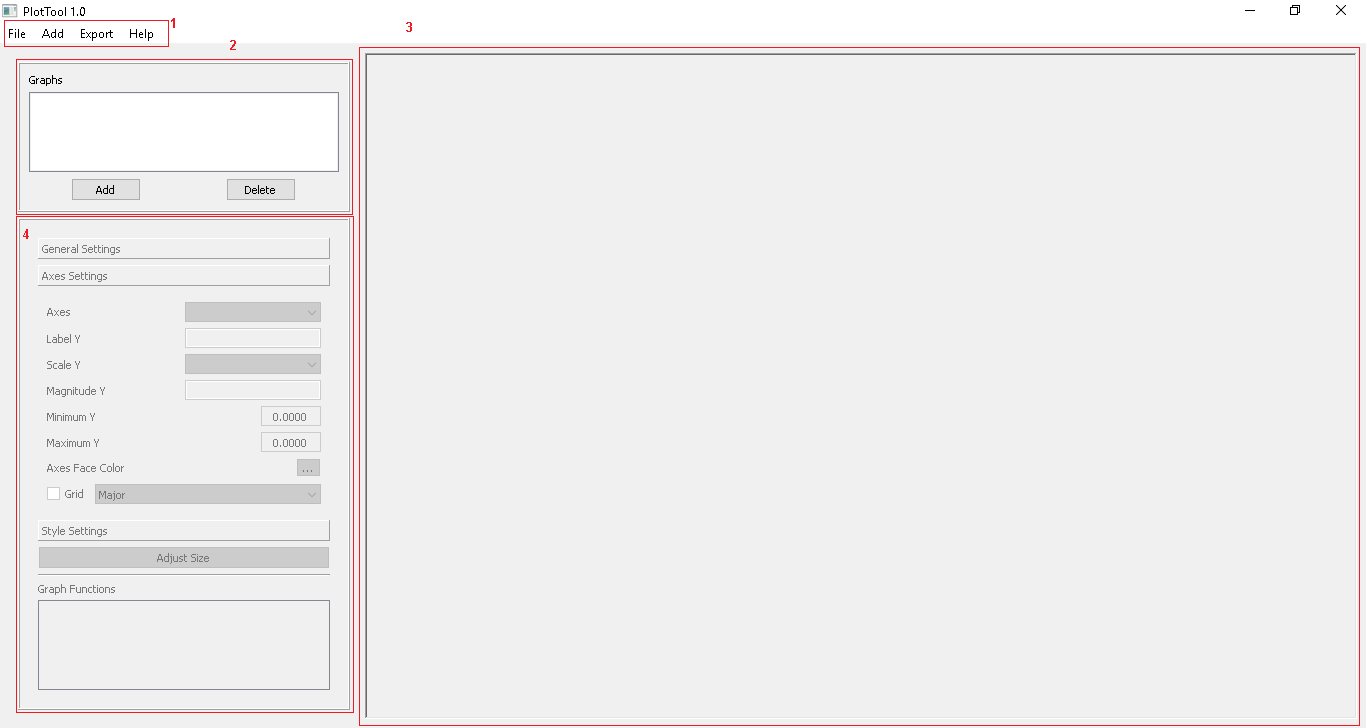
\includegraphics[scale=0.5]{resources/initial_window.png}
	\caption{Ventana principal del inicio del programa}
	\label{fig:initial_window}
	\end{center}
\end{figure}

\subsection{Men\'u de opciones}

\subsubsection{File}
La opci\'on del men\'u File permite al usuario abrir y/o guardar el Graph seleccionado, almacenando los datos del
mismo para que puedan volver a ser abiertos. Vale aclarar que s\'olo se guarda su descripci\'on como gr\'afico y no la customizaci\'on de la salida.

\subsubsection{Add}
La opci\'on del men\'u Add permite al usuario agregar diferentes entradas al Graph actual, internamente el programa est\'a estructurado de forma escalable permitiendo a\~nadir a futuro nuevas funcionalidas u opciones para la incorporaci\'on de datos al Graph. En el momento de la realizaci\'on de este manual, se disponen de las
opciones Signals, Transfer Function, from LTSpice y from Excel.

\begin{figure}[H]
	\begin{center}
	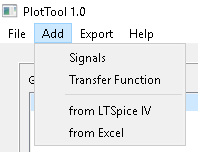
\includegraphics[scale=0.8]{resources/menu_add.png}
	\caption{Menu Add, agregando GraphFunctions al Graph actual.}
	\end{center}
\end{figure}

\subsubsection{Export}
La opci\'on del men\'u Export permite al usuario exportar el Graph sobre el cual est\'a trabajando en un archivo
de formato de salida como lo es .png. De igual modo que se mencion\'o antes, resultar\'ia sencillo agregar nuevas funcionalidades garantizando un mayor rango de opciones de salida.

\begin{figure}[H]
	\begin{center}
	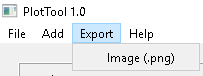
\includegraphics[scale=0.8]{resources/menu_export.png}
	\caption{Menu Export, exportar como .png el Graph actual.}
	\end{center}
\end{figure}

\subsection{Lista de Graphs}
La lista de Graphs creados permite seleccionar sobre cu\'al se encuentra trabajando actualmente el usuario y es indispensable para determinar sobre qu\'e Graph se aplican los cambios que se operan con cualquiera de las herramientas del programa que se ir\'an describiendo a lo largo de la gu\'ia. En la creaci\'on de un nuevo Graph
es necesario destinar un nombre al mismo y una magnitud.

\begin{figure}[H]
\begin{center}
	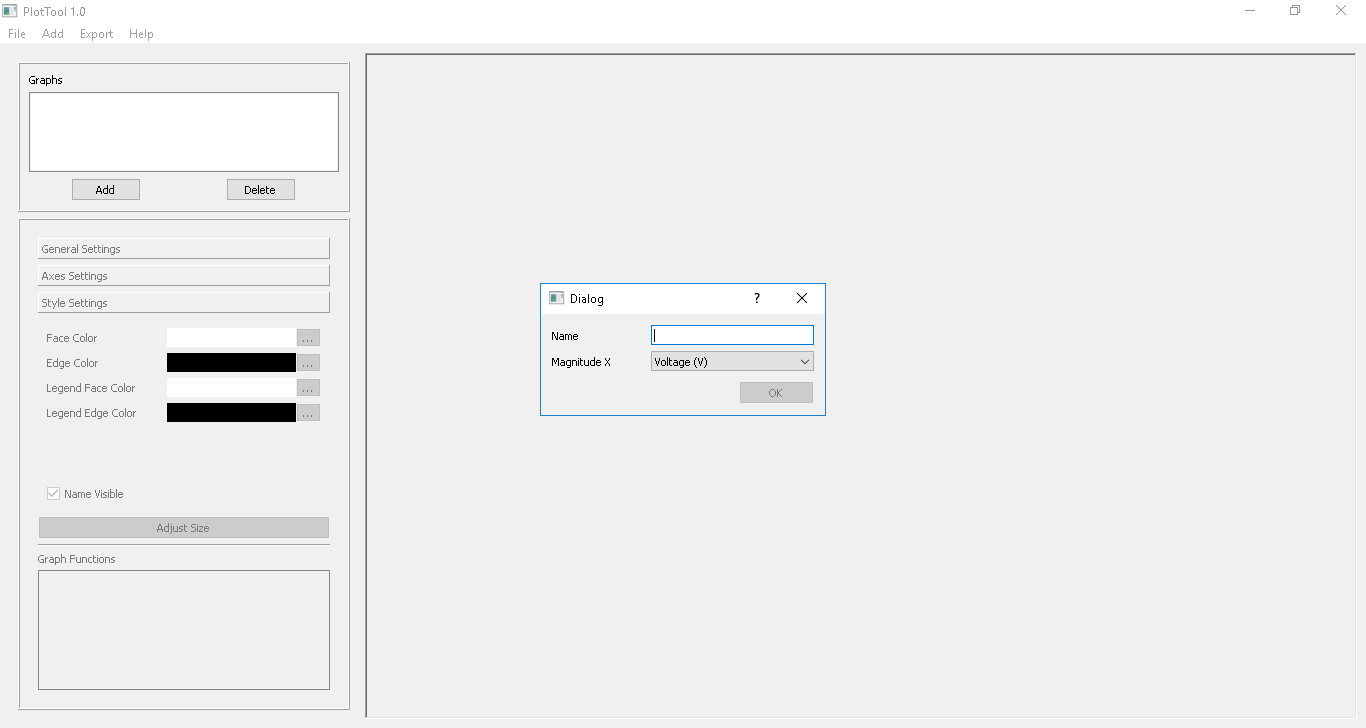
\includegraphics[scale=0.5]{resources/example_create_plotter.png}
	\caption{Creaci\'on de una Graph}
\end{center}
\end{figure}

\subsection{Visor de propiedades}
El visor de propiedades es una parte elemental del programa pues permite modificar las propiedades del Graph, tanto su nombre, como muchas de sus caracter\'isticas, algunas de ellas relativas al estilo de la salida. Es importante mencionar que en todos ellos se puede observar que dentro del visor de propiedades hay una lista que contiene los GraphFunctions que refieren a las entradas que fueron agregadas al gr\'afico, permitiendo determinar si son visible, borrarlas, cambiarles el nombre, el color, entre otras cosas.

\begin{figure}[H]
\begin{center}
	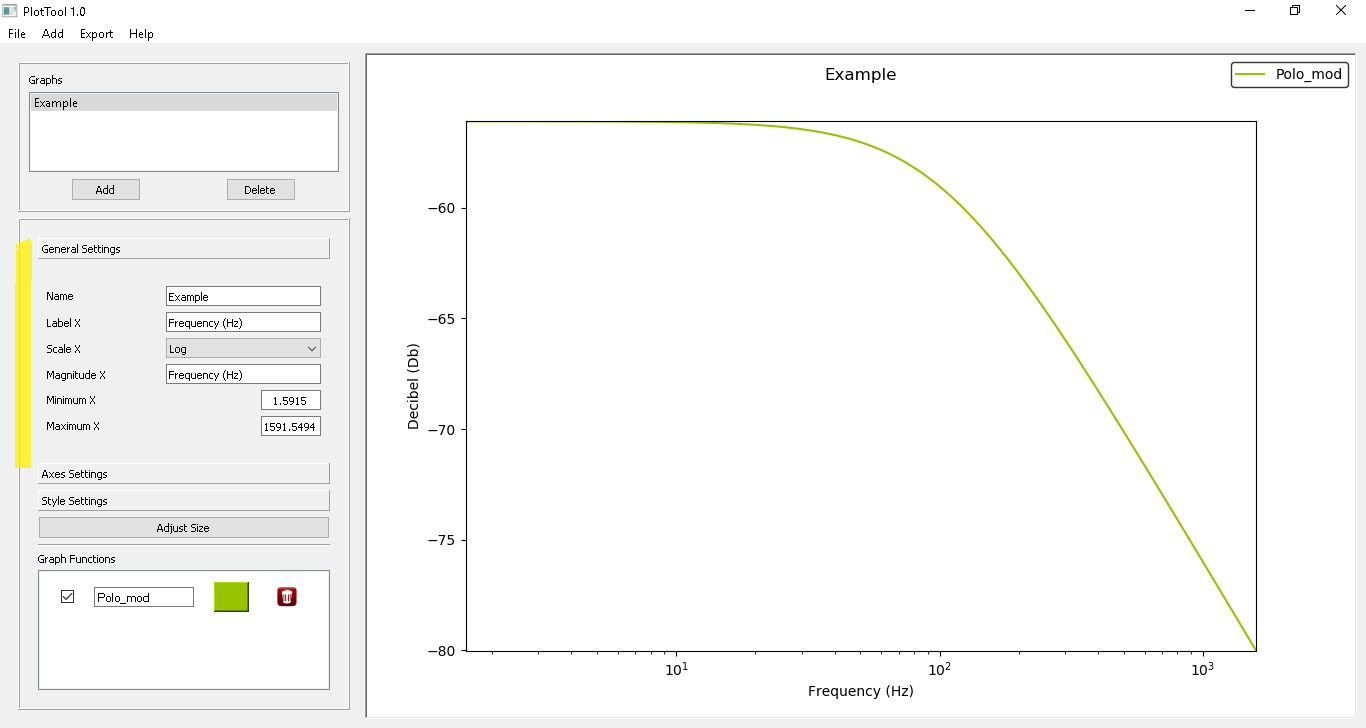
\includegraphics[scale=0.5]{resources/visor_general.png}
	\caption{General settings}
\end{center}
\end{figure}

\begin{figure}[H]
\begin{center}
	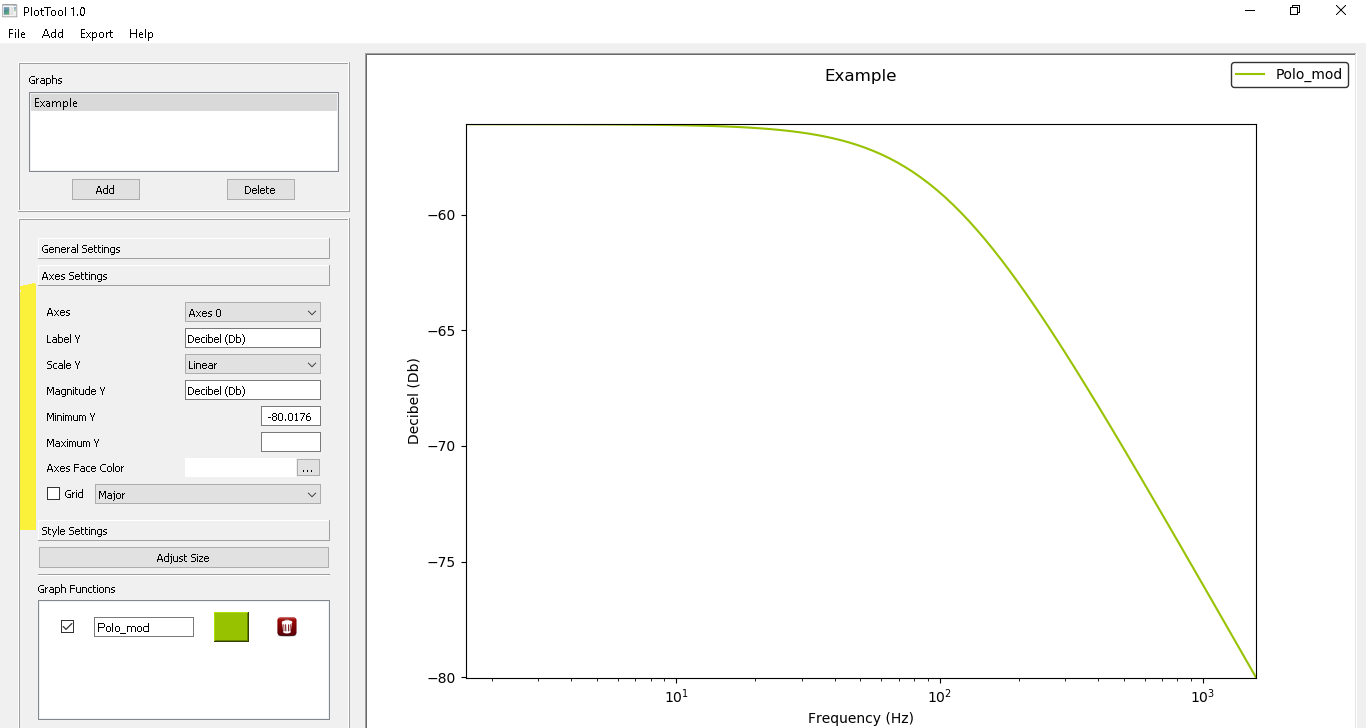
\includegraphics[scale=0.5]{resources/visor_axes.png}
	\caption{Axes settings}
\end{center}
\end{figure}

\begin{figure}[H]
\begin{center}
	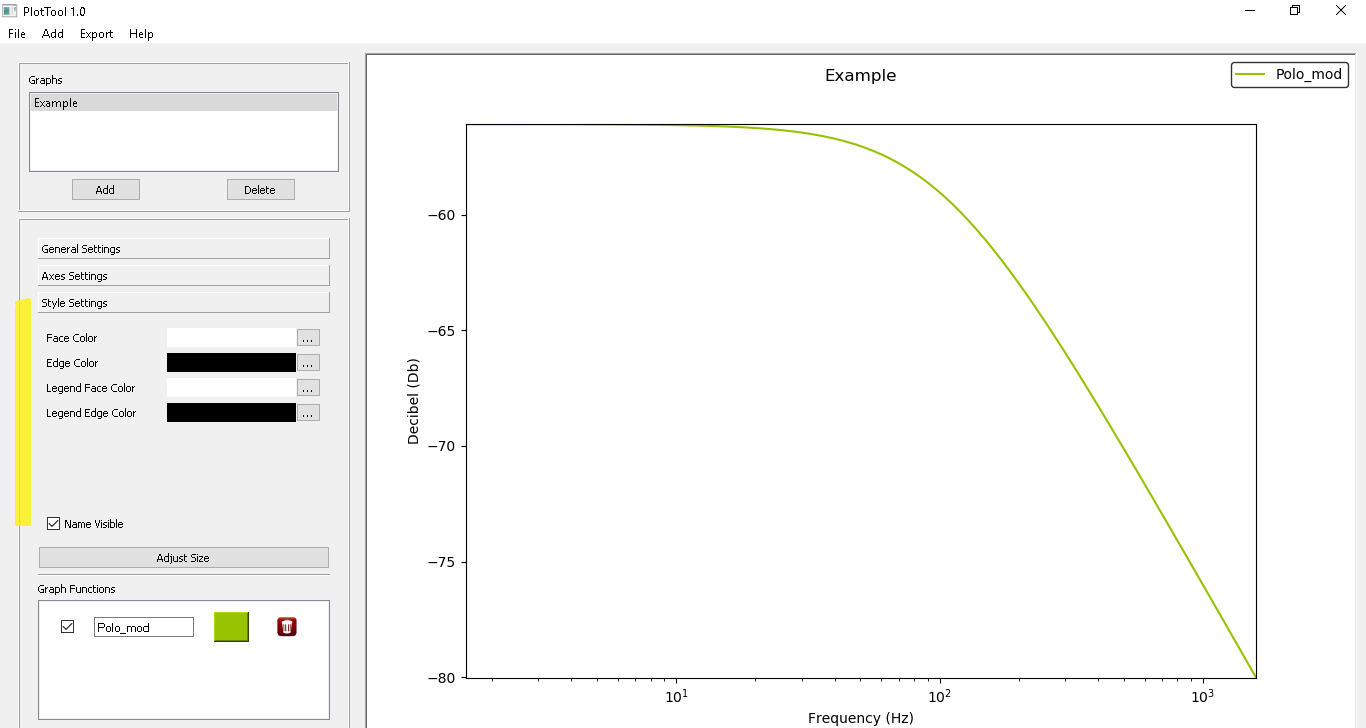
\includegraphics[scale=0.5]{resources/visor_style.png}
	\caption{Style settings}
\end{center}
\end{figure}

\end{document}